\documentclass[xcolor=x11names,compress]{beamer}

%% General document %%%%%%%%%%%%%%%%%%%%%%%%%%%%%%%%%%
\usepackage{graphicx}
\usepackage{svg}
\usepackage{amsfonts}
\usepackage{tikz}
\usetikzlibrary{decorations.fractals}
\usetikzlibrary{arrows.meta}
\usetikzlibrary{3d}
\usetikzlibrary{positioning}
\usetikzlibrary{fit}
\usetikzlibrary{shapes}
\usetikzlibrary{shapes.geometric}
\usetikzlibrary{shapes.misc}
\usetikzlibrary{backgrounds}
\usetikzlibrary{arrows.meta}
%%%%%%%%%%%%%%%%%%%%%%%%%%%%%%%%%%%%%%%%%%%%%%%%%%%%%%


%% Beamer Layout %%%%%%%%%%%%%%%%%%%%%%%%%%%%%%%%%%
\useoutertheme[subsection=false,shadow]{miniframes}
\useinnertheme{default}
\usefonttheme{serif}
\usepackage{palatino}
\usepackage{setspace,textcomp,soul}
\usepackage{beamerprosper}

\setbeamerfont{title like}{shape=\scshape}
\setbeamerfont{frametitle}{shape=\scshape}
\definecolor{bluUnicam}{RGB}{27,43,74}
\definecolor{redUnicam}{RGB}{219,0,36}
\definecolor{orangeUnicam}{RGB}{234,114,40}
\setbeamercolor*{lower separation line head}{bg=redUnicam}
\setbeamercolor*{normal text}{fg=bluUnicam,bg=white}
\setbeamercolor*{alerted text}{fg=red}
\setbeamercolor*{example text}{fg=black}
\setbeamercolor*{structure}{fg=orangeUnicam}
\setbeamercolor*{frametitle}{fg=redUnicam}

\setbeamercolor*{palette secondary}{fg=orangeUnicam,bg=bluUnicam}
\setbeamercolor*{palette tertiary}{fg=orangeUnicam,bg=bluUnicam}
\setbeamercolor*{palette quaternary}{fg=black,bg=black!10}


% Add navigation symbols at the bottom
\setbeamertemplate{navigation symbols}{} % remove default navigation symbols
\setbeamertemplate{footline}{%
    \leavevmode%
    \hbox{%
        \begin{beamercolorbox}[wd=\paperwidth, ht=1ex,dp=1ex,center]{author in head/foot}%
            \usebeamerfont{author in head/foot}
        \end{beamercolorbox}}%
}

\newtheorem{esempio}{Esempio}\theoremstyle{definition}
\newtheorem{definizione}{Definizione} \theoremstyle{plain}
\newtheorem{teorema}{Teorema}

%%%%%%%%%%%%%%%%%%%%%%%%%%%%%%%%%%%%%%%%%%%%%%%%%%

\begin{document}

% Intro
%%%%%%%%%%%%%%%%%%%%%%%%%%%%%%%%%%%%%%%%%%%%%%%%%%%%%%
%%%%%%%%%%%%%%%%%%%%%%%%%%%%%%%%%%%%%%%%%%%%%%%%%%%%%%
    %\usebackgroundtemplate{
\includegraphics[width=\paperwidth,height=\paperheight]{./immagini/thanks}}
\begin{frame}
\title{\color{redUnicam}{Progettazione di una Struttura Dati per Rappresentare e Analizzare \\ Collezioni di Sogni}}
%\subtitle{SUBTITLE}
\begin{center}

\author{{\textbf{Marco Caputo}}\\
\fontsize{8pt}{10}\selectfont{marco.caputo@studenti.unicam.it}}
\institute{
%\fontsize{6pt}{6}\selectfont{Università di Camerino}
\begin{figure}[htpb!]
   	
\includegraphics[width=0.10\textwidth]{immagini/stemma}
    \end{figure}}
\date{22 Luglio 2024}
\titlepage
\end{center}
\end{frame}

\section{\scshape Definizioni}
%%%%%%%%%%%%%%%%%%%%%%%%%%%%%%%%%%%%%%%%%%%%%%%%%%%%%%
%%%%%%%%%%%%%%%%%%%%%%%%%%%%%%%%%%%%%%%%%%%%%%%%%%%%%%
\begin{frame}[t]{Contrazione di Grafi}
    \begin{minipage}[t]{\textwidth}
        \begin{minipage}[t]{0.46\textwidth}
    \centering
    Contrazione di archi
    \parbox{0.1\textwidth}{\vspace*{0.75cm}}
    \resizebox{\textwidth}{!}{
        \begin{tikzpicture}
  % Styles for the nodes and edges
  \tikzstyle{vertex} = [draw, circle, inner sep=2pt, minimum size=12pt]
  \tikzstyle{edge} = [->, >={Stealth[round]}, thick]

  % Left Graph
  \node[vertex, label=left:u] (u) at (0, 1) {};
  \node[] (u2) at (-0.2, 0.8) {};
  \node[vertex, label=left:v] (v) at (0, -1) {};
  \node[] (v2) at (-0.2, -0.8) {};

  \node[vertex] (a) at (-1.5, 0.5) {};
  \node[vertex] (b) at (1.5, 0.5) {};
  \node[vertex] (c) at (-0.5, 2.2) {};
  \node[vertex] (d) at (1, 1.5) {};
  \node[vertex] (e) at (-1, -2) {};
  \node[vertex] (f) at (1.5, -0.7) {};
  \node[vertex] (g) at (0.5, -2.2) {};

  \draw[edge] (u) -- (a);
  \draw[edge] (u) -- (b);
  \draw[edge] (c) -- (u);
  \draw[edge] (u) -- (d);
  \draw[edge] (f) -- (u);
  \draw[edge] (c) -- (a);

  \draw[edge] (v) -- (a);
  \draw[edge] (e) -- (v);
  \draw[edge] (v) -- (f);
  \draw[edge] (v) -- (g);
  \draw[edge] (g) -- (e);

  \draw[edge] (u) -- (v);
  \draw[->, red] (u2) -- ++( 0, -0.5);
  \draw[->, red] (v2) -- ++( 0, 0.5);

  % Right Graph
  \node[vertex, label=left:w] (w) at (6, 0) {};

  \node[vertex] (a2) at (4.5, 0.5) {};
  \node[vertex] (b2) at (7.5, 0.5) {};
  \node[vertex] (c2) at (5.5, 2.2) {};
  \node[vertex] (d2) at (7, 1.5) {};
  \node[vertex] (e2) at (5, -2) {};
  \node[vertex] (f2) at (7.5, -0.7) {};
  \node[vertex] (g2) at (6.5, -2.2) {};

  \draw[edge] (w) -- (a2);
  \draw[edge] (w) -- (b2);
  \draw[edge] (c2) -- (w);
  \draw[edge] (w) -- (d2);
  \draw[edge] (f2) -- (w);
  \draw[edge] (c2) -- (a2);

  \draw[edge] (w) -- (a2);
  \draw[edge] (e2) -- (w);
  \draw[edge] (w) -- (f2);
  \draw[edge] (w) -- (g2);
  \draw[edge] (g2) -- (e2);

\end{tikzpicture}
    }
\end{minipage}
    \end{minipage}
\end{frame}

%%%%%%%%%%%%%%%%%%%%%%%%%%%%%%%%%%%%%%%%%%%%%%%%%%%%%%
%%%%%%%%%%%%%%%%%%%%%%%%%%%%%%%%%%%%%%%%%%%%%%%%%%%%%%
\begin{frame}[t]{Contrazione di Grafi}
    \vspace*{-0.65cm}
    \begin{minipage}[t]{\textwidth}
        \begin{minipage}[t]{0.46\textwidth}
    \centering
    Contrazione di archi
    \parbox{0.1\textwidth}{\vspace*{0.75cm}}
    \resizebox{\textwidth}{!}{
        \begin{tikzpicture}
  % Styles for the nodes and edges
  \tikzstyle{vertex} = [draw, circle, inner sep=2pt, minimum size=12pt]
  \tikzstyle{edge} = [->, >={Stealth[round]}, thick]

  % Left Graph
  \node[vertex, label=left:u] (u) at (0, 1) {};
  \node[] (u2) at (-0.2, 0.8) {};
  \node[vertex, label=left:v] (v) at (0, -1) {};
  \node[] (v2) at (-0.2, -0.8) {};

  \node[vertex] (a) at (-1.5, 0.5) {};
  \node[vertex] (b) at (1.5, 0.5) {};
  \node[vertex] (c) at (-0.5, 2.2) {};
  \node[vertex] (d) at (1, 1.5) {};
  \node[vertex] (e) at (-1, -2) {};
  \node[vertex] (f) at (1.5, -0.7) {};
  \node[vertex] (g) at (0.5, -2.2) {};

  \draw[edge] (u) -- (a);
  \draw[edge] (u) -- (b);
  \draw[edge] (c) -- (u);
  \draw[edge] (u) -- (d);
  \draw[edge] (f) -- (u);
  \draw[edge] (c) -- (a);

  \draw[edge] (v) -- (a);
  \draw[edge] (e) -- (v);
  \draw[edge] (v) -- (f);
  \draw[edge] (v) -- (g);
  \draw[edge] (g) -- (e);

  \draw[edge] (u) -- (v);
  \draw[->, red] (u2) -- ++( 0, -0.5);
  \draw[->, red] (v2) -- ++( 0, 0.5);

  % Right Graph
  \node[vertex, label=left:w] (w) at (6, 0) {};

  \node[vertex] (a2) at (4.5, 0.5) {};
  \node[vertex] (b2) at (7.5, 0.5) {};
  \node[vertex] (c2) at (5.5, 2.2) {};
  \node[vertex] (d2) at (7, 1.5) {};
  \node[vertex] (e2) at (5, -2) {};
  \node[vertex] (f2) at (7.5, -0.7) {};
  \node[vertex] (g2) at (6.5, -2.2) {};

  \draw[edge] (w) -- (a2);
  \draw[edge] (w) -- (b2);
  \draw[edge] (c2) -- (w);
  \draw[edge] (w) -- (d2);
  \draw[edge] (f2) -- (w);
  \draw[edge] (c2) -- (a2);

  \draw[edge] (w) -- (a2);
  \draw[edge] (e2) -- (w);
  \draw[edge] (w) -- (f2);
  \draw[edge] (w) -- (g2);
  \draw[edge] (g2) -- (e2);

\end{tikzpicture}
    }
\end{minipage}
        \hfill
        \begin{minipage}[t]{0.46\textwidth}
    \centering
    Contrazione di sottografi
    \parbox{0.1\textwidth}{\vspace*{2cm}}
    \resizebox{\textwidth}{!}{
        \begin{tikzpicture}[scale=1.5]

% Define the styles for the nodes and edges
\tikzstyle{vertex} = [draw, circle, inner sep=2pt, minimum size=18pt]
\tikzstyle{edge} = [->, >={Stealth[round]}, thick]
\tikzset{thick vertex/.style = {draw, circle, inner sep=2pt, minimum size=18pt, line width=1.7pt}}]
\tikzset{thick edge/.style = {->, >={Stealth[round]}, line width=1.7pt}}

% Left graph
\node[] (g) at (3.2,1.8) {$G$};

\node[thick vertex] (v1) at (0,0) {$v_1$};
\node[thick vertex] (v2) at (0,2) {$v_2$};
\node[thick vertex] (v3) at (0.75,1) {$v_3$};
\node[thick vertex] (v4) at (1.5,0) {$v_4$};
\node[vertex] (v5) at (1.5,2) {$v_5$};
\node[vertex] (v6) at (2.5,0) {$v_6$};
\node[vertex] (v7) at (2.5,2) {$v_7$};
\node[vertex] (v8) at (3.2,1) {$v_8$};

% Draw edges for left graph
\draw[thick edge] (v1) -- (v2);
\draw[thick edge] (v1) -- (v3);
\draw[thick edge] (v2) -- (v3);
\draw[thick edge] (v3) -- (v4);
\draw[thick edge] (v4) -- (v1);
\draw[edge] (v2) -- (v5);
\draw[edge] (v3) -- (v5);
\draw[edge] (v4) -- (v5);
\draw[edge] (v4) -- (v6);
\draw[edge] (v5) -- (v7);
\draw[edge] (v6) -- (v7);
\draw[edge] (v6) -- (v8);
\draw[edge] (v7) -- (v4);
\draw[edge] (v7) -- (v8);
\draw[edge] (v6) -- (v8);

% Right graph
\node[] (g2) at (8.2,1.8) {$G'$};

\node[thick vertex] (w) at (5.8,0.7) {$w$};
\node[vertex] (v5) at (6.5,2) {$v_5$};
\node[vertex] (v6) at (7.5,0) {$v_6$};
\node[vertex] (v7) at (7.5,2) {$v_7$};
\node[vertex] (v8) at (8.2,1) {$v_8$};

% Draw edges for right graph
\draw[edge] (w) -- (v5);
\draw[edge] (w) -- (v6);
\draw[edge] (v5) -- (v7);
\draw[edge] (v6) -- (v7);
\draw[edge] (v6) -- (v8);
\draw[edge] (v7) -- (w);
\draw[edge] (v7) -- (v8);
\draw[edge] (v6) -- (v8);

% Draw the arrow
\draw[-{Stealth[length=3mm, width=2mm]}, thick] (4,1.1) -- (5,1.1);

\end{tikzpicture}
    }
\end{minipage}
    \end{minipage}
\end{frame}

%%%%%%%%%%%%%%%%%%%%%%%%%%%%%%%%%%%%%%%%%%%%%%%%%%%%%%
%%%%%%%%%%%%%%%%%%%%%%%%%%%%%%%%%%%%%%%%%%%%%%%%%%%%%%
\begin{frame}[t]{Contrazione di Grafi}
    \vspace*{-0.65cm}
    \begin{minipage}[t]{\textwidth}
        \begin{minipage}[t]{0.46\textwidth}
    \centering
    Contrazione di archi
    \parbox{0.1\textwidth}{\vspace*{0.75cm}}
    \resizebox{\textwidth}{!}{
        \begin{tikzpicture}
  % Styles for the nodes and edges
  \tikzstyle{vertex} = [draw, circle, inner sep=2pt, minimum size=12pt]
  \tikzstyle{edge} = [->, >={Stealth[round]}, thick]

  % Left Graph
  \node[vertex, label=left:u] (u) at (0, 1) {};
  \node[] (u2) at (-0.2, 0.8) {};
  \node[vertex, label=left:v] (v) at (0, -1) {};
  \node[] (v2) at (-0.2, -0.8) {};

  \node[vertex] (a) at (-1.5, 0.5) {};
  \node[vertex] (b) at (1.5, 0.5) {};
  \node[vertex] (c) at (-0.5, 2.2) {};
  \node[vertex] (d) at (1, 1.5) {};
  \node[vertex] (e) at (-1, -2) {};
  \node[vertex] (f) at (1.5, -0.7) {};
  \node[vertex] (g) at (0.5, -2.2) {};

  \draw[edge] (u) -- (a);
  \draw[edge] (u) -- (b);
  \draw[edge] (c) -- (u);
  \draw[edge] (u) -- (d);
  \draw[edge] (f) -- (u);
  \draw[edge] (c) -- (a);

  \draw[edge] (v) -- (a);
  \draw[edge] (e) -- (v);
  \draw[edge] (v) -- (f);
  \draw[edge] (v) -- (g);
  \draw[edge] (g) -- (e);

  \draw[edge] (u) -- (v);
  \draw[->, red] (u2) -- ++( 0, -0.5);
  \draw[->, red] (v2) -- ++( 0, 0.5);

  % Right Graph
  \node[vertex, label=left:w] (w) at (6, 0) {};

  \node[vertex] (a2) at (4.5, 0.5) {};
  \node[vertex] (b2) at (7.5, 0.5) {};
  \node[vertex] (c2) at (5.5, 2.2) {};
  \node[vertex] (d2) at (7, 1.5) {};
  \node[vertex] (e2) at (5, -2) {};
  \node[vertex] (f2) at (7.5, -0.7) {};
  \node[vertex] (g2) at (6.5, -2.2) {};

  \draw[edge] (w) -- (a2);
  \draw[edge] (w) -- (b2);
  \draw[edge] (c2) -- (w);
  \draw[edge] (w) -- (d2);
  \draw[edge] (f2) -- (w);
  \draw[edge] (c2) -- (a2);

  \draw[edge] (w) -- (a2);
  \draw[edge] (e2) -- (w);
  \draw[edge] (w) -- (f2);
  \draw[edge] (w) -- (g2);
  \draw[edge] (g2) -- (e2);

\end{tikzpicture}
    }
\end{minipage}
        \hfill
        \begin{minipage}[t]{0.46\textwidth}
    \centering
    Contrazione di sottografi
    \parbox{0.1\textwidth}{\vspace*{2cm}}
    \resizebox{\textwidth}{!}{
        \begin{tikzpicture}[scale=1.5]

% Define the styles for the nodes and edges
\tikzstyle{vertex} = [draw, circle, inner sep=2pt, minimum size=18pt]
\tikzstyle{edge} = [->, >={Stealth[round]}, thick]
\tikzset{thick vertex/.style = {draw, circle, inner sep=2pt, minimum size=18pt, line width=1.7pt}}]
\tikzset{thick edge/.style = {->, >={Stealth[round]}, line width=1.7pt}}

% Left graph
\node[] (g) at (3.2,1.8) {$G$};

\node[thick vertex] (v1) at (0,0) {$v_1$};
\node[thick vertex] (v2) at (0,2) {$v_2$};
\node[thick vertex] (v3) at (0.75,1) {$v_3$};
\node[thick vertex] (v4) at (1.5,0) {$v_4$};
\node[vertex] (v5) at (1.5,2) {$v_5$};
\node[vertex] (v6) at (2.5,0) {$v_6$};
\node[vertex] (v7) at (2.5,2) {$v_7$};
\node[vertex] (v8) at (3.2,1) {$v_8$};

% Draw edges for left graph
\draw[thick edge] (v1) -- (v2);
\draw[thick edge] (v1) -- (v3);
\draw[thick edge] (v2) -- (v3);
\draw[thick edge] (v3) -- (v4);
\draw[thick edge] (v4) -- (v1);
\draw[edge] (v2) -- (v5);
\draw[edge] (v3) -- (v5);
\draw[edge] (v4) -- (v5);
\draw[edge] (v4) -- (v6);
\draw[edge] (v5) -- (v7);
\draw[edge] (v6) -- (v7);
\draw[edge] (v6) -- (v8);
\draw[edge] (v7) -- (v4);
\draw[edge] (v7) -- (v8);
\draw[edge] (v6) -- (v8);

% Right graph
\node[] (g2) at (8.2,1.8) {$G'$};

\node[thick vertex] (w) at (5.8,0.7) {$w$};
\node[vertex] (v5) at (6.5,2) {$v_5$};
\node[vertex] (v6) at (7.5,0) {$v_6$};
\node[vertex] (v7) at (7.5,2) {$v_7$};
\node[vertex] (v8) at (8.2,1) {$v_8$};

% Draw edges for right graph
\draw[edge] (w) -- (v5);
\draw[edge] (w) -- (v6);
\draw[edge] (v5) -- (v7);
\draw[edge] (v6) -- (v7);
\draw[edge] (v6) -- (v8);
\draw[edge] (v7) -- (w);
\draw[edge] (v7) -- (v8);
\draw[edge] (v6) -- (v8);

% Draw the arrow
\draw[-{Stealth[length=3mm, width=2mm]}, thick] (4,1.1) -- (5,1.1);

\end{tikzpicture}
    }
\end{minipage}
    \end{minipage}
    \begin{minipage}[t]{\textwidth}
    \vspace{0.5cm}
    \centering
    Grafo quoziente \\
    \resizebox{0.6\textwidth}{!}{
        \vspace*{0.5cm}
        \begin{tikzpicture}[x=0.75pt,y=0.75pt,yscale=-1,xscale=1,graph node/.style={circle, draw, inner sep=2pt}, >={Stealth}]
%uncomment if require: \path (0,193); %set diagram left start at 0, and has height of 193

%Shape: Ellipse [id:dp5716078870574002]
\draw   (157.72,126.37) .. controls (157.72,122.18) and (161.11,118.78) .. (165.3,118.78) .. controls (169.49,118.78) and (172.89,122.18) .. (172.89,126.37) .. controls (172.89,130.56) and (169.49,133.96) .. (165.3,133.96) .. controls (161.11,133.96) and (157.72,130.56) .. (157.72,126.37) -- cycle ;
%Straight Lines [id:da030036293703488592]
\draw    (162.59,132.58) -- (119.64,155.58) ;
\draw [shift={(117,157)}, rotate = 331.82] [fill={rgb, 255:red, 0; green, 0; blue, 0 }  ][line width=0.08]  [draw opacity=0] (7.14,-3.43) -- (0,0) -- (7.14,3.43) -- cycle    ;
%Shape: Ellipse [id:dp4694008742489806]
\draw   (96.69,48.05) .. controls (96.69,43.86) and (100.09,40.46) .. (104.28,40.46) .. controls (108.47,40.46) and (111.87,43.86) .. (111.87,48.05) .. controls (111.87,52.24) and (108.47,55.64) .. (104.28,55.64) .. controls (100.09,55.64) and (96.69,52.24) .. (96.69,48.05) -- cycle ;
%Shape: Ellipse [id:dp43075157044098433]
\draw   (157.8,159.08) .. controls (157.8,154.89) and (161.2,151.49) .. (165.39,151.49) .. controls (169.58,151.49) and (172.98,154.89) .. (172.98,159.08) .. controls (172.98,163.27) and (169.58,166.67) .. (165.39,166.67) .. controls (161.2,166.67) and (157.8,163.27) .. (157.8,159.08) -- cycle ;
%Straight Lines [id:da7735175864839863]
\draw    (157.8,159.08) -- (122.91,161.4) ;
\draw [shift={(119.91,161.6)}, rotate = 356.19] [fill={rgb, 255:red, 0; green, 0; blue, 0 }  ][line width=0.08]  [draw opacity=0] (7.14,-3.43) -- (0,0) -- (7.14,3.43) -- cycle    ;
%Shape: Ellipse [id:dp8331515179192863]
\draw   (103.74,126.6) .. controls (103.74,122.41) and (107.14,119.01) .. (111.33,119.01) .. controls (115.52,119.01) and (118.91,122.41) .. (118.91,126.6) .. controls (118.91,130.79) and (115.52,134.19) .. (111.33,134.19) .. controls (107.14,134.19) and (103.74,130.79) .. (103.74,126.6) -- cycle ;
%Straight Lines [id:da8805781538281761]
\draw    (165.3,133.96) -- (165.38,148.49) ;
\draw [shift={(165.39,151.49)}, rotate = 269.72] [fill={rgb, 255:red, 0; green, 0; blue, 0 }  ][line width=0.08]  [draw opacity=0] (7.14,-3.43) -- (0,0) -- (7.14,3.43) -- cycle    ;
%Shape: Ellipse [id:dp11540879760206746]
\draw   (24.41,89.59) .. controls (24.41,85.4) and (27.81,82) .. (32,82) .. controls (36.19,82) and (39.59,85.4) .. (39.59,89.59) .. controls (39.59,93.78) and (36.19,97.17) .. (32,97.17) .. controls (27.81,97.17) and (24.41,93.78) .. (24.41,89.59) -- cycle ;
%Straight Lines [id:da7303103534852602]
\draw    (90.93,73.6) -- (90.93,73.6) -- (59.6,55.5) ;
\draw [shift={(57,54)}, rotate = 30.02] [fill={rgb, 255:red, 0; green, 0; blue, 0 }  ][line width=0.08]  [draw opacity=0] (7.14,-3.43) -- (0,0) -- (7.14,3.43) -- cycle    ;
%Shape: Ellipse [id:dp18097418973582324]
\draw   (42.46,49.02) .. controls (42.46,44.83) and (45.85,41.43) .. (50.04,41.43) .. controls (54.23,41.43) and (57.63,44.83) .. (57.63,49.02) .. controls (57.63,53.21) and (54.23,56.6) .. (50.04,56.6) .. controls (45.85,56.6) and (42.46,53.21) .. (42.46,49.02) -- cycle ;
%Straight Lines [id:da4155132765855869]
\draw    (57.63,49.02) -- (93.69,48.12) ;
\draw [shift={(96.69,48.05)}, rotate = 178.58] [fill={rgb, 255:red, 0; green, 0; blue, 0 }  ][line width=0.08]  [draw opacity=0] (7.14,-3.43) -- (0,0) -- (7.14,3.43) -- cycle    ;
%Straight Lines [id:da1262374391562433]
\draw    (32,82) -- (44.09,57.83) ;
\draw [shift={(45.43,55.14)}, rotate = 116.57] [fill={rgb, 255:red, 0; green, 0; blue, 0 }  ][line width=0.08]  [draw opacity=0] (7.14,-3.43) -- (0,0) -- (7.14,3.43) -- cycle    ;
%Straight Lines [id:da572291236631852]
\draw    (105.14,120.57) -- (78.69,87.9) -- (54.94,58.92) ;
\draw [shift={(53.04,56.6)}, rotate = 50.66] [fill={rgb, 255:red, 0; green, 0; blue, 0 }  ][line width=0.08]  [draw opacity=0] (7.14,-3.43) -- (0,0) -- (7.14,3.43) -- cycle    ;
%Curve Lines [id:da021365012814849704]
\draw    (98.95,42.72) .. controls (89.68,35.14) and (74.55,33.42) .. (61.85,39.48) .. controls (60.82,39.97) and (59.81,40.51) .. (58.82,41.1) ;
\draw [shift={(56.34,42.72)}, rotate = 324.46] [fill={rgb, 255:red, 0; green, 0; blue, 0 }  ][line width=0.08]  [draw opacity=0] (7.14,-3.43) -- (0,0) -- (7.14,3.43) -- cycle    ;
%Shape: Ellipse [id:dp776996888716095]
\draw   (90.41,78.59) .. controls (90.41,74.4) and (93.81,71) .. (98,71) .. controls (102.19,71) and (105.59,74.4) .. (105.59,78.59) .. controls (105.59,82.78) and (102.19,86.17) .. (98,86.17) .. controls (93.81,86.17) and (90.41,82.78) .. (90.41,78.59) -- cycle ;
%Shape: Ellipse [id:dp46756955428949243]
\draw   (104.74,161.6) .. controls (104.74,157.41) and (108.14,154.01) .. (112.33,154.01) .. controls (116.52,154.01) and (119.91,157.41) .. (119.91,161.6) .. controls (119.91,165.79) and (116.52,169.19) .. (112.33,169.19) .. controls (108.14,169.19) and (104.74,165.79) .. (104.74,161.6) -- cycle ;
%Straight Lines [id:da11987408246874143]
\draw    (112.33,154.01) -- (111.48,137.18) ;
\draw [shift={(111.33,134.19)}, rotate = 87.11] [fill=bluUnicam][line width=0.08]  [draw opacity=0] (7.14,-3.43) -- (0,0) -- (7.14,3.43) -- cycle    ;
%Straight Lines [id:da7165440164643189]
\draw    (118.91,126.6) -- (154.72,126.39) ;
\draw [shift={(157.72,126.37)}, rotate = 179.66] [fill=bluUnicam][line width=0.08]  [draw opacity=0] (7.14,-3.43) -- (0,0) -- (7.14,3.43) -- cycle    ;
%Straight Lines [id:da8702436048031414]
\draw    (106.33,156.19) -- (39.27,97.97) ;
\draw [shift={(37,96)}, rotate = 40.96] [fill=bluUnicam][line width=0.08]  [draw opacity=0] (7.14,-3.43) -- (0,0) -- (7.14,3.43) -- cycle    ;
%Straight Lines [id:da01851647212321983]
\draw    (111.33,119.01) -- (101.88,88.04) ;
\draw [shift={(101,85.17)}, rotate = 73.03] [fill=bluUnicam][line width=0.08]  [draw opacity=0] (7.14,-3.43) -- (0,0) -- (7.14,3.43) -- cycle    ;
%Shape: Ellipse [id:dp5733943324242119]
\draw   (194.69,42.05) .. controls (194.69,37.86) and (198.09,34.46) .. (202.28,34.46) .. controls (206.47,34.46) and (209.87,37.86) .. (209.87,42.05) .. controls (209.87,46.24) and (206.47,49.64) .. (202.28,49.64) .. controls (198.09,49.64) and (194.69,46.24) .. (194.69,42.05) -- cycle ;
%Shape: Ellipse [id:dp4982173340393281]
\draw   (198.69,97.05) .. controls (198.69,92.86) and (202.09,89.46) .. (206.28,89.46) .. controls (210.47,89.46) and (213.87,92.86) .. (213.87,97.05) .. controls (213.87,101.24) and (210.47,104.64) .. (206.28,104.64) .. controls (202.09,104.64) and (198.69,101.24) .. (198.69,97.05) -- cycle ;
%Shape: Ellipse [id:dp6443249330347911]
\draw   (145.69,58.05) .. controls (145.69,53.86) and (149.09,50.46) .. (153.28,50.46) .. controls (157.47,50.46) and (160.87,53.86) .. (160.87,58.05) .. controls (160.87,62.24) and (157.47,65.64) .. (153.28,65.64) .. controls (149.09,65.64) and (145.69,62.24) .. (145.69,58.05) -- cycle ;
%Shape: Ellipse [id:dp2962874847585506]
\draw   (151.69,79.05) .. controls (151.69,74.86) and (155.09,71.46) .. (159.28,71.46) .. controls (163.47,71.46) and (166.87,74.86) .. (166.87,79.05) .. controls (166.87,83.24) and (163.47,86.64) .. (159.28,86.64) .. controls (155.09,86.64) and (151.69,83.24) .. (151.69,79.05) -- cycle ;
%Straight Lines [id:da08505254887451863]
\draw    (198.69,94.05) -- (168.68,83.08) ;
\draw [shift={(165.87,82.05)}, rotate = 20.08] [fill=bluUnicam][line width=0.08]  [draw opacity=0] (7.14,-3.43) -- (0,0) -- (7.14,3.43) -- cycle    ;
%Straight Lines [id:da8488856387468098]
\draw    (105.59,78.59) -- (148.69,79.02) ;
\draw [shift={(151.69,79.05)}, rotate = 180.57] [fill=bluUnicam][line width=0.08]  [draw opacity=0] (7.14,-3.43) -- (0,0) -- (7.14,3.43) -- cycle    ;
%Straight Lines [id:da9679144897377887]
\draw    (145.69,58.05) -- (105.98,71.6) ;
\draw [shift={(103.14,72.57)}, rotate = 341.16] [fill=bluUnicam][line width=0.08]  [draw opacity=0] (7.14,-3.43) -- (0,0) -- (7.14,3.43) -- cycle    ;
%Straight Lines [id:da895747160462798]
\draw    (194.69,42.05) -- (114.86,47.83) ;
\draw [shift={(111.87,48.05)}, rotate = 355.86] [fill=bluUnicam][line width=0.08]  [draw opacity=0] (7.14,-3.43) -- (0,0) -- (7.14,3.43) -- cycle    ;
%Straight Lines [id:da9678052539321507]
\draw    (195.69,45.05) -- (163.73,55.15) ;
\draw [shift={(160.87,56.05)}, rotate = 342.47] [fill=bluUnicam][line width=0.08]  [draw opacity=0] (7.14,-3.43) -- (0,0) -- (7.14,3.43) -- cycle    ;
%Straight Lines [id:da12597861271491162]
\draw    (202.28,49.64) -- (205.98,86.48) ;
\draw [shift={(206.28,89.46)}, rotate = 264.26] [fill=bluUnicam][line width=0.08]  [draw opacity=0] (7.14,-3.43) -- (0,0) -- (7.14,3.43) -- cycle    ;
%Straight Lines [id:da05573449739087133]
\draw    (197.14,47.57) -- (166.5,71.71) ;
\draw [shift={(164.14,73.57)}, rotate = 321.77] [fill=bluUnicam][line width=0.08]  [draw opacity=0] (7.14,-3.43) -- (0,0) -- (7.14,3.43) -- cycle    ;
%Shape: Ellipse [id:dp18633067687908644]
\draw  [color=bluUnicam  ,draw opacity=1 ][line width=1]  (2.14,95.57) .. controls (2.14,43.66) and (58.55,1.57) .. (128.14,1.57) .. controls (197.73,1.57) and (254.14,43.66) .. (254.14,95.57) .. controls (254.14,147.49) and (197.73,189.57) .. (128.14,189.57) .. controls (58.55,189.57) and (2.14,147.49) .. (2.14,95.57) -- cycle ;
%Curve Lines [id:da9916896653167908]
\draw [color=bluUnicam  ,draw opacity=1 ][line width=1]    (30.14,154.57) .. controls (79.86,141.57) and (142.86,99.57) .. (133.86,2) ;
%Curve Lines [id:da16207253703394464]
\draw [color=bluUnicam  ,draw opacity=1 ][line width=1]    (234,146.57) .. controls (224.86,122.57) and (151.86,96.57) .. (115,94.57) ;

% Text Node
\draw (19,16) node [anchor=north west][inner sep=0.75pt]    {$\textcolor{bluUnicam}{\mathbf{A}}$};
% Text Node
\draw (228,16) node [anchor=north west][inner sep=0.75pt]    {$\textcolor{bluUnicam}{\mathbf{B}}$};
% Text Node
\draw (217,168.4) node [anchor=north west][inner sep=0.75pt]    {$\textcolor{bluUnicam}{\mathbf{C}}$};


% Define nodes in the condensed graph
\node[graph node, fill=bluUnicam!20, draw=black] (A) at (340,100) {A};
\node[graph node, fill=bluUnicam!20, draw=black] (B) at (400,50) {B};
\node[graph node, fill=bluUnicam!20, draw=black] (C) at (400,150) {C};

% Draw edges in the quotient graph
\draw[->, thick] (A) to[out=0, in=90] (B);
\draw[->, thick] (B) to[out=180, in=270] (A);
\draw[->, thick] (A) -- (C);

% Draw the arrow
\draw[-{Stealth[length=3mm, width=2mm]}, orangeUnicam, thick, dashed] (270,100) -- (310,100);

\end{tikzpicture}
    }
\end{minipage}
\end{frame}

%%%%%%%%%%%%%%%%%%%%%%%%%%%%%%%%%%%%%%%%%%%%%%%%%%%%%%
%%%%%%%%%%%%%%%%%%%%%%%%%%%%%%%%%%%%%%%%%%%%%%%%%%%%%%
\begin{frame}[t]{Grafo multi-livello}
    \vspace{-0.5cm}
    \begin{minipage}[t]{\textwidth}
\begin{definizione}[Grafo multi-livello]
    Un \textbf{grafo multi-livello} $M$ \`e una coppia $(G, \Gamma)$ dove:
        \begin{itemize}
            \item $G = (V, E)$ \`e un grafo;
            \item $\Gamma = \langle \, f_{C_1}, f_{C_2}, .., f_{C_k} \rangle$ \`e una sequenza di funzioni di contrazione.
        \end{itemize}
    \end{definizione}
\end{minipage}
\end{frame}

%%%%%%%%%%%%%%%%%%%%%%%%%%%%%%%%%%%%%%%%%%%%%%%%%%%%%%
%%%%%%%%%%%%%%%%%%%%%%%%%%%%%%%%%%%%%%%%%%%%%%%%%%%%%%
\begin{frame}[t]{Grafo multi-livello}
    \vspace{-0.5cm}
    \begin{minipage}[t]{\textwidth}
\begin{definizione}[Grafo multi-livello]
    Un \textbf{grafo multi-livello} $M$ \`e una coppia $(G, \Gamma)$ dove:
        \begin{itemize}
            \item $G = (V, E)$ \`e un grafo;
            \item $\Gamma = \langle \, f_{C_1}, f_{C_2}, .., f_{C_k} \rangle$ \`e una sequenza di funzioni di contrazione.
        \end{itemize}
    \end{definizione}
\end{minipage}
    \begin{minipage}[t]{\textwidth}
    \vspace{0.3cm}
    \begin{figure}
        \centering
        \resizebox{0.5\textwidth}{!}{
            \begin{tikzpicture}[x={(1cm,0cm)},y={(0cm,1cm)},z={(0.410cm,0.300cm)}]
    \node[canvas is zy plane at x=0,draw,fill=white] (g0) at (0,0) {
    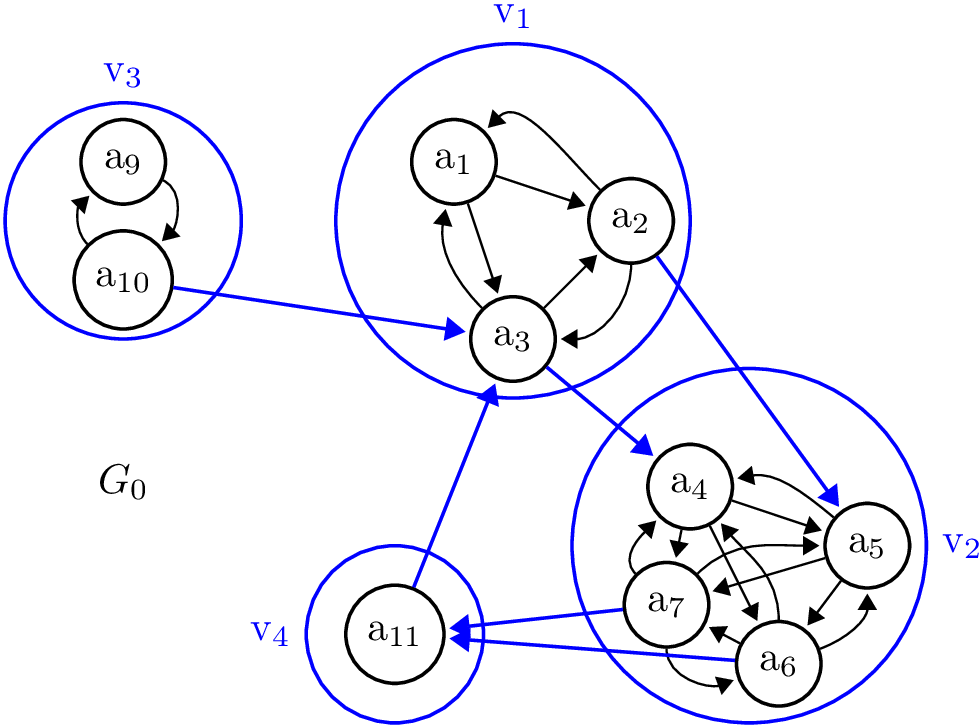
\includegraphics[scale=0.315]{immagini/graph0.png}
    };
    \node[canvas is zy plane at x=5,draw,fill=white] (g1) at (0,0) {
        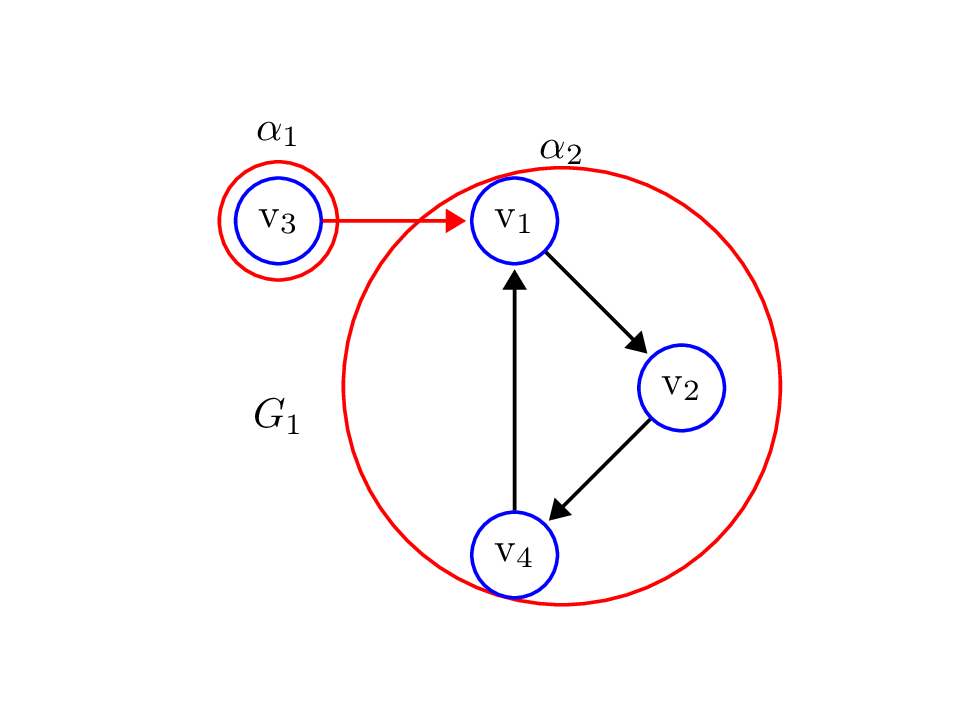
\includegraphics[scale=0.315]{immagini/graph1.png}
    };
    \node[canvas is zy plane at x=10,draw,fill=white] (g2) at (0,0) {
        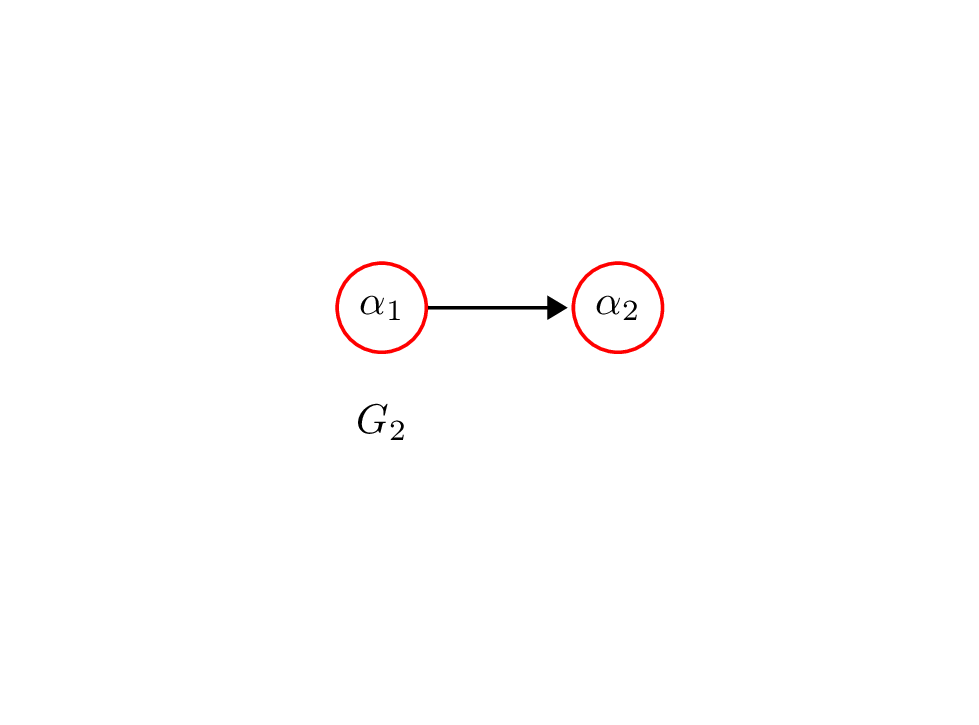
\includegraphics[scale=0.315]{immagini/graph2.png}
    };

    \node (G0) [below of=g0, node distance=5.2cm] {\huge $G_0$};
    \node (G1) [below of=g1, node distance=5.2cm] {\huge $G_1$};
    \node (G2) [below of=g2, node distance=5.2cm] {\huge $G_2$};

    \node (G0d) [below of=G0, node distance=1cm] {};
    \node (G1d) [below of=G1, node distance=1cm] {};
    \node (G2d) [below of=G2, node distance=1cm] {};

    \draw[->, line width=2pt, redUnicam] (G0d) -- (G1d) node[midway, below, red] {\huge $f_{C_1}$};
    \draw[->, line width=2pt, redUnicam] (G1d) -- (G2d) node[midway, below, red] {\huge $f_{C_2}$};
\end{tikzpicture}
        }
    \end{figure}
\end{minipage}
\end{frame}

%%%%%%%%%%%%%%%%%%%%%%%%%%%%%%%%%%%%%%%%%%%%%%%%%%%%%%
%%%%%%%%%%%%%%%%%%%%%%%%%%%%%%%%%%%%%%%%%%%%%%%%%%%%%%
\begin{frame}[t]{Grafo decontraibile}
    \vspace{-0.5cm}
    \begin{minipage}[t]{\textwidth}
    {\tiny
    \begin{definizione}[Grafo decontraibile]
    Un \textbf{grafo decontraibile} \`e una quadrupla $G = (V, E, dec_V, dec_E)$ dove:
    \begin{itemize}
        \item $V$ \`e un insieme di elementi detti \textbf{supernodi};
        \item $E \subseteq V \times V$ \`e un insieme di coppie ordinate di supernodi, dette \textbf{superarchi};
        \item $dec_V : V \rightarrow \mathcal{G}_D$ \`e una funzione tale per cui $dec_V(v) = (\mathcal{V}_v,
            \mathcal{E}_v, dec_{\mathcal{V}_v}, dec_{\mathcal{E}_v})$ \`e un grafo decontraibile rappresentato
            dal supernodo $v$;
        \item $dec_E : E \rightarrow (\mathcal{V} \times \mathcal{V})$ con $\mathcal{V} = \bigcup_{v \in V}\mathcal{V}_v$,
            \`e una funzione tale per cui $\forall$ $ e = (u, v)$, $dec_E(e) = \mathcal{E}_e \subseteq$ $\{(a, b)$ $\mid$ $a \in \mathcal{V}_u$ $\wedge$
            $b \in \mathcal{V}_v\}$ \`e un insieme di archi rappresentati dal superarco $e$.
    \end{itemize}
    \end{definizione}}
\end{minipage}
\end{frame}

%%%%%%%%%%%%%%%%%%%%%%%%%%%%%%%%%%%%%%%%%%%%%%%%%%%%%%
%%%%%%%%%%%%%%%%%%%%%%%%%%%%%%%%%%%%%%%%%%%%%%%%%%%%%%
\begin{frame}[t]{Grafo decontraibile}
    \vspace{-0.5cm}
    \begin{minipage}[t]{\textwidth}
    {\tiny
    \begin{definizione}[Grafo decontraibile]
    Un \textbf{grafo decontraibile} \`e una quadrupla $G = (V, E, dec_V, dec_E)$ dove:
    \begin{itemize}
        \item $V$ \`e un insieme di elementi detti \textbf{supernodi};
        \item $E \subseteq V \times V$ \`e un insieme di coppie ordinate di supernodi, dette \textbf{superarchi};
        \item $dec_V : V \rightarrow \mathcal{G}_D$ \`e una funzione tale per cui $dec_V(v) = (\mathcal{V}_v,
            \mathcal{E}_v, dec_{\mathcal{V}_v}, dec_{\mathcal{E}_v})$ \`e un grafo decontraibile rappresentato
            dal supernodo $v$;
        \item $dec_E : E \rightarrow (\mathcal{V} \times \mathcal{V})$ con $\mathcal{V} = \bigcup_{v \in V}\mathcal{V}_v$,
            \`e una funzione tale per cui $\forall$ $ e = (u, v)$, $dec_E(e) = \mathcal{E}_e \subseteq$ $\{(a, b)$ $\mid$ $a \in \mathcal{V}_u$ $\wedge$
            $b \in \mathcal{V}_v\}$ \`e un insieme di archi rappresentati dal superarco $e$.
    \end{itemize}
    \end{definizione}}
\end{minipage}
    \begin{minipage}[t]{\textwidth}
        \vspace{0.25cm}
        \centering
        \resizebox{0.6\textwidth}{!}{
        \begin{tikzpicture}
[mynode/.style={draw, thick, circle, size=0.3mm}, ->,shorten >=1pt,auto,node distance=2cm, thick,
  main node/.style={circle,draw}, little node/.style={circle,draw, minimum size=7.5mm, inner sep=0mm}]

% Nodes
  \node[main node] (A) {$v_1$};
  \node[main node, bluUnicam] (B) [right of=A] {$v_2$};
  \node[main node, bluUnicam] (C) [below right of=B] {$v_3$};
  \node[main node] (D) [below left of=C] {$v_4$};

  % Edges
  \path[every node/.style={font=\sffamily\small}]
    (A) edge node [above] {$e_1$} (B)
    (B) edge[bluUnicam] node [right, name=e2] {$e_2$} (C)
    (C) edge node [below] {$e_3$} (D)
    (B) edge node [left] {$e_4$} (D);

  % G_v2 graph
  \begin{scope}[shift={(6,1)}]
    \draw[bluUnicam] (0,0) circle (1.5cm);
    \node[little node, bluUnicam] (X) at (-0.5,0.5) {$a_1$};
    \node[little node, bluUnicam] (Y) at (1,0) {$a_2$};
    \node[little node, bluUnicam] (Z) at (0,-1) {$a_3$};
    \path[every node/.style={font=\sffamily\small}]
      (X) edge[bluUnicam] (Y)
      (Y) edge[bluUnicam] (Z)
      (Z) edge[bluUnicam] (X);
  \end{scope}

  % Link
  \draw[dashed, line width=1.5pt, red] (B) to[out=65, in=145] node[midway, above, sloped, red] {$dec_{V}(v_2)$} (4.5,1);

% G_v3 graph
  \begin{scope}[shift={(8,-2.5)}]
    \draw[blue] (0,0) circle (1.5cm);
    \node[little node, blue] (T) at (-0.5,0.5) {$a_4$};
    \node[little node, blue] (U) at (1,0) {$a_5$};
    \node[little node, blue] (V) at (0.25,-1) {$a_6$};
    \node[little node, blue] (W) at (-0.5,-0.5) {$a_7$};
    \path[every node/.style={font=\sffamily\small}]
      (U) edge[blue] (T)
      (U) edge[blue] (W)
      (U) edge[blue] (V);
  \end{scope}

  % Link
\draw[dashed, line width=1.5pt, red] (C) to[out=300, in=145] node[midway, below, sloped, red] {$dec_{V}(v_3)$} (6.5,-2);
  \end{tikzpicture}
        }
\end{minipage}
\end{frame}

%%%%%%%%%%%%%%%%%%%%%%%%%%%%%%%%%%%%%%%%%%%%%%%%%%%%%%
%%%%%%%%%%%%%%%%%%%%%%%%%%%%%%%%%%%%%%%%%%%%%%%%%%%%%%
\begin{frame}[t]{Grafo decontraibile}
    \vspace{-0.5cm}
    \begin{minipage}[t]{\textwidth}
    {\tiny
    \begin{definizione}[Grafo decontraibile]
    Un \textbf{grafo decontraibile} \`e una quadrupla $G = (V, E, dec_V, dec_E)$ dove:
    \begin{itemize}
        \item $V$ \`e un insieme di elementi detti \textbf{supernodi};
        \item $E \subseteq V \times V$ \`e un insieme di coppie ordinate di supernodi, dette \textbf{superarchi};
        \item $dec_V : V \rightarrow \mathcal{G}_D$ \`e una funzione tale per cui $dec_V(v) = (\mathcal{V}_v,
            \mathcal{E}_v, dec_{\mathcal{V}_v}, dec_{\mathcal{E}_v})$ \`e un grafo decontraibile rappresentato
            dal supernodo $v$;
        \item $dec_E : E \rightarrow (\mathcal{V} \times \mathcal{V})$ con $\mathcal{V} = \bigcup_{v \in V}\mathcal{V}_v$,
            \`e una funzione tale per cui $\forall$ $ e = (u, v)$, $dec_E(e) = \mathcal{E}_e \subseteq$ $\{(a, b)$ $\mid$ $a \in \mathcal{V}_u$ $\wedge$
            $b \in \mathcal{V}_v\}$ \`e un insieme di archi rappresentati dal superarco $e$.
    \end{itemize}
    \end{definizione}}
\end{minipage}
    \begin{minipage}[t]{\textwidth}
        \vspace{0.25cm}
        \centering
        \resizebox{0.6\textwidth}{!}{
        \begin{tikzpicture}
[mynode/.style={draw, thick, circle, size=0.3mm}, ->,shorten >=1pt,auto,node distance=2cm, thick,
  main node/.style={circle,draw}, little node/.style={circle,draw, minimum size=7.5mm, inner sep=0mm}]

% Nodes
  \node[main node] (A) {$v_1$};
  \node[main node, orangeUnicam] (B) [right of=A] {$v_2$};
  \node[main node, orangeUnicam] (C) [below right of=B] {$v_3$};
  \node[main node] (D) [below left of=C] {$v_4$};

  % Edges
  \path[every node/.style={font=\sffamily\small}]
    (A) edge node [above] {$e_1$} (B)
    (B) edge[orangeUnicam] node [right, name=e2] {$e_2$} (C)
    (C) edge node [below] {$e_3$} (D)
    (B) edge node [left] {$e_4$} (D);

  % G_v2 graph
  \begin{scope}[shift={(6,1)}]
    \draw[orangeUnicam] (0,0) circle (1.5cm);
    \node[little node] (X) at (-0.5,0.5) {$a_1$};
    \node[little node] (Y) at (1,0) {$a_2$};
    \node[little node] (Z) at (0,-1) {$a_3$};
    \path[every node/.style={font=\sffamily\small}]
      (X) edge[black] (Y)
      (Y) edge[black] (Z)
      (Z) edge[black] (X);
  \end{scope}

  % Link
  \draw[dashed, line width=1.5pt, red] (B) to[out=65, in=145] node[midway, above, sloped, red] {$dec_{V}(v_2)$} (4.5,1);

% G_v3 graph
  \begin{scope}[shift={(8,-2.5)}]
    \draw[orangeUnicam] (0,0) circle (1.5cm);
    \node[little node] (T) at (-0.5,0.5) {$a_4$};
    \node[little node] (U) at (1,0) {$a_5$};
    \node[little node] (V) at (0.25,-1) {$a_6$};
    \node[little node] (W) at (-0.5,-0.5) {$a_7$};
    \path[every node/.style={font=\sffamily\small}]
      (U) edge[black] (T)
      (U) edge[black] (W)
      (U) edge[black] (V);
  \end{scope}

  % Link
\draw[dashed, line width=1.5pt, red] (C) to[out=300, in=145] node[midway, below, sloped, red] {$dec_{V}(v_3)$} (6.5,-2);

% Edges between graphs
  \path[orangeUnicam]
    (Z) edge[orangeUnicam] (T)
    (Y) edge[orangeUnicam] (U);

  % Links
\draw[dashed, line width=1.5pt, red] (e2) to[out=0, in=155] node[midway, below, sloped, red] {$dec_{E}(e_2)$} (6.75,-1);
\draw[dashed, line width=1.5pt, red] (e2) to[out=0, in=175] (8,-0.7);
  \end{tikzpicture}
        }
\end{minipage}
\end{frame}

%%%%%%%%%%%%%%%%%%%%%%%%%%%%%%%%%%%%%%%%%%%%%%%%%%%%%%
%%%%%%%%%%%%%%%%%%%%%%%%%%%%%%%%%%%%%%%%%%%%%%%%%%%%%%
\section*{Acknowledgements}
\begin{frame}{Acknowledgements}
\begin{center}

\includegraphics[width=6.5cm]{./immagini/thanks}
\end{center}
\end{frame}

\end{document}
